\section{Grid Computing}
Grid computing is a type of computing infrastructure where multiple computers work together to achieve a common goal. Unused resources from multiple computers are utilised together to perform a task that is usually extremely large or to solve complex problems, which would otherwise be too demanding for a single computer. Resources such as processing power, storage, and memory are shared across multiple machines. Grid computing has several applications, some of which are analysing designs, performing simulations, financial services, and weather modelling.\cite{AWS_grid_computing}

Computers or servers on a grid are called nodes. There is no limit to the number of nodes a grid can have. There are three types of nodes. These nodes are referred to as master nodes, worker nodes, and user nodes, in this report. There is also middleware, which is a computer program that connects different computers in a grid system together. It helps manage how much processing power each node uses and ensures that no single node utilises too much as this could cause problems for other nodes. The grid middleware can also provide security and prevent nodes from misusing the resources. Often the middleware would be located on the master node, where it is used to assign tasks to the other nodes in the system. 

A worker node is a node that provides computational power to help in the grid. The user node is the one requesting help with a task, that is provided to the grid, as shown in figure \ref{fig:Grid computing illustration} as either a desktop or laptop PC. The user node sends a task it wants fulfilled to the master node which is in the centre \cite{AWS_grid_computing}. Subsequently, as depicted in the illustration, the master node distributes the task to the nodes located in the upper, right, and lower locations, highlighting that the task is distributed throughout the system. 

\begin{figure}[H]
    \centering
    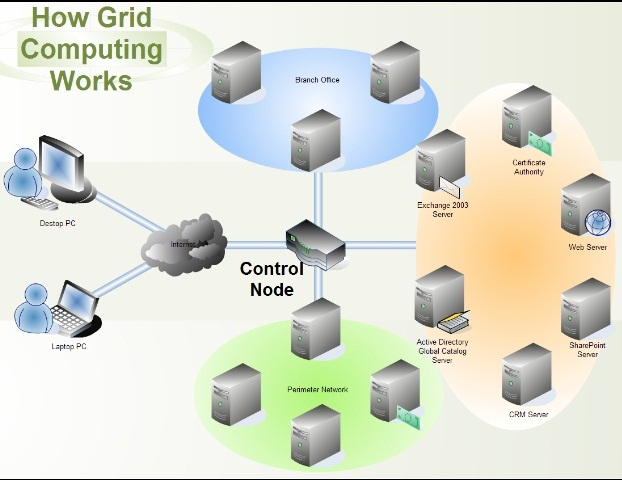
\includegraphics[scale=0.60]{figures/Grid-Computing.jpg}
    \caption{ 
    A visualisation of what a grid computing system could look like. In this illustration, the Master node is called Control node \cite{Gridcomputing_image}.}
    \label{fig:Grid computing illustration}
\end{figure}

When creating a grid computing system, there are several factors that need to be fulfilled to have an optimal system. When assessing how optimal the system is, it is important to keep the limits that the system needs to work within in mind. For example, if running time is important, one would need to set a limit for the time the system is allowed to run for. This is referred to as temporal verification.
Other things that are relevant to optimise are structure verification, performance verification, and resource verification.

Structure verification refers to the verification of the system's structure and the way the system is set up. This includes both the semantic and syntactic structure of a given system. The syntactic part of the system includes problems such as lack of synchronisation, general misuse of the structure, deadlock, where some nodes are effectively blocking each other since they are trying to reach each other's resources, and livelock, where the nodes are constantly changing their own output, since the other node that it needs work from changes.
The semantic part is also important. Suppose a system works in terms of syntax and a task needs to be done in either node A or B, but the semantics of the system decide that node C, even though it is nonexistent, would be a better option. For the structural integrity of the system, it is important to avoid such a scenario \cite{grid_workflow_validation}.

Another thing that needs to be verified in the system is its performance. This is called the verification process, where the system is tested within user-defined parameters, such as an average completion time, average capacity, synchronisation delay, average resource allocation, and so on. This can be tested either on each node in the system or on the whole system in general. There are multiple ways, this can be achieved, such as the Markovian chain theory, the queuing theory, or simulation tools, with each their advantages and disadvantages \cite{grid_workflow_validation}.

Another type of verification that is important to have in the system, is resource verification. This is a process where the system is tested to ensure that it distributes the data that it gets efficiently and the resources of the system are handled correctly. Ensuring that nodes are not trying to compute the same data and that the resources are not distributed to the same node \cite{grid_workflow_validation}.